% === T03 - Tiempos, Simulación y Verificación ===
% David Alejandro Gonzalez Marquez
% fokerman@gmail.com
% https://github.com/fokerman/fpgaSoftcoreProgrammingCourse

\RequirePackage[2020-02-02]{latexrelease}

\documentclass[aspectratio=169]{beamer}
\usepackage{../packages}

\newcommand{\na}{\cellcolor{naranjauca}}
\newcommand{\gm}{\cellcolor{gray!50}} 

\title{\Huge Tiempos, Simulación y Verificación}
\author{David Alejandro González Márquez}
\institute{Programación de softcores en FPGAs\\
Programa de Profesoras/es Visitantes\\
Departamento de computación\\
Universidad de Buenos Aires}


\date{}

\lstset{
  backgroundcolor=\color{gray!20},   % choose the background color; you must add \usepackage{color} or \usepackage{xcolor}; should come as last argument
  basicstyle=\footnotesize,        % the size of the fonts that are used for the code
  breakatwhitespace=false,         % sets if automatic breaks should only happen at whitespace
  breaklines=true,                 % sets automatic line breaking
  extendedchars=true,              % lets you use non-ASCII characters; for 8-bits encodings only, does not work with UTF-8
  keepspaces=true,                 % keeps spaces in text, useful for keeping indentation of code (possibly needs columns=flexible)
  language=Verilog,                 % the language of the code
  showspaces=false,                % show spaces everywhere adding particular underscores; it overrides 'showstringspaces'
  showstringspaces=false,          % underline spaces within strings only
  showtabs=false,                  % show tabs within strings adding particular underscores
  tabsize=2,	                   % sets default tabsize to 2 spaces
  frame=single	                   % adds a frame around the code // topline bottomline leftline
}

\begin{document}

\begin{frame}[plain]
    \titlepage
    \begin{textblock}{110}(25,80)
    \begin{tcolorbox}[size=small,width=\textwidth,colback={gray!30},title={}]
    \begin{center}
     \scriptsize Clase disponible en: \url{https://github.com/fokerman/fpgaSoftcoreProgrammingCourse}
    \end{center}
    \end{tcolorbox}
    \end{textblock}
\end{frame}

\begin{frame}[fragile]
    \frametitle{Tiempos, Simulación y Verificación} 
    \textcolor{naranjauca}{1 - Temporización de circuitos combinacionales}
    \begin{itemize}
     \item Propagación de señales.
     \item Aparición de \emph{glitches}.
    \end{itemize}
    \bigskip
    \textcolor{naranjauca}{2 - Temporización de circuitos secuenciales}
    \begin{itemize}
     \item Tiempo entre cambios, tiempo de espera y tiempo en que se mantienen los datos.
     \item Determinación de la velocidad máxima de operación.
    \end{itemize}
    \bigskip
    \textcolor{naranjauca}{3 - Verificación de circuitos}
    \begin{itemize}
     \item Verificación funcional y temporal.
     \item Construcción de tests.
    \end{itemize}
\end{frame}

\begin{frame}[fragile]
    \frametitle{Concesiones en el diseño de circuitos}
    \uncover<1->{
    \textcolor{naranjauca}{\textbf{Área}}\\
    \begin{itemize}
    \item \small El área utilizada es \textbf{proporcional al costo} del dispositivo, cuanta más área requerida,\\ más costoso de construir es el circuito.
    \end{itemize}
    }
    \uncover<2->{
    \textcolor{naranjauca}{\textbf{Speed/Througput}}\\
    \begin{itemize}
    \item \small Circuitos más rápidos y con más capacidad, implican \textbf{más componentes}, más complejidad,\\ mayor consumo.
    \end{itemize}
    }
    \uncover<3->{
    \textcolor{naranjauca}{\textbf{Power/Energy}}\\
    \begin{itemize}
    \item \small Buscamos circuitos que consuman energía de forma \textbf{eficiente} para la tarea a realizar.
    \item \small Dispositivos de alto rendimiento deben poder \textbf{disipar} mucha energía.
    \item \small Dispositivos móviles tienen una cantidad \textbf{limitada} de energía disponible.
    \end{itemize}
    }
    \uncover<4->{
    \textcolor{naranjauca}{\textbf{Design Time}}\\
    \begin{itemize}
    \item \small Los diseños más complejos requieren más \textbf{tiempo de diseño}, repercutiendo en costos.
    \item \small Además el diseño debe considera el \emph{time to market} del circuito como \textbf{producto}.
    \end{itemize}
    }
\end{frame}

\begin{frame}[fragile]
    \frametitle{Tiempos en un circuito (\emph{Circuit Timming})}
    \textcolor{naranjauca}{Timing}\\
    Consiste en el análisis de la temporización de las operaciones que se suceden dentro de un circuito digital.\\
    \bigskip
    \pause
    \textcolor{gray}{Busca responder}\\
    \begin{center}
    ¿Qué tan rápido puede ser mi circuito?\\
    \pause
    ¿Puedo hacer correr aun más rápido mi circuito?\\
    \pause
    ¿Qué sucede si supero el límite de mi circuito?\\
    \pause
    \end{center}
    \bigskip
    \textcolor{verdeuca}{Un diseño puede ser logicamente correcto, pero puede fallar en una implementación por problemas fisicos de llevar este circuito a la vida real.
    \textbf{El \emph{timing} es uno de estos problemas}.}
\end{frame}

\begin{frame}[fragile,t]
    \frametitle{Modelo de los circuitos digitales}
    Podemos modelar problemas considerando que los cambios en las entradas de las compuertas se ven inmediatamente reflejados en la salida.\\
    \textcolor{verdeuca}{Esta es una muy conveniente abstracción, pero dista de modelar que sucede en el mundo físico.}\\
    \bigskip
    \uncover<2->{
    En la vida real tenemos retardos (\textcolor{naranjauca}{\emph{delay}}):
    \begin{itemize}
    \item Las salidas demoran tiempo en \textbf{exponer los cambios} de las entradas.
    \item Los transistores toman un \textbf{tiempo finito} en cambiar.
    \item Las señales demoran en \textbf{propagarse por los cables}.
    \end{itemize}
    }
    \uncover<3->{
    \bigskip
    \begin{tabular}[]{ccp{4cm}}
        \includegraphics[scale=1]{img/circuito_retardo-layer1.pdf} &
        \includegraphics[scale=1]{img/circuito_retardo-layer3.pdf} \\
    \end{tabular}
    }
    \begin{textblock}{45}(103,59)
    \uncover<3->{
    \small
    $\text{x}$: Rango de tiempo en que esperamos recibir la respuesta. Desde que comienza a cambiar hasta que efectivamente cambia.
    }
    \end{textblock}
\end{frame}

\begin{frame}[fragile]
    \frametitle{Variaciones del \emph{delay} en un circuito}
    \small
    \textcolor{naranjauca}{Las causas del \emph{delay} son:}\\
    \begin{itemize}
    \item La \textbf{capacitancia} y \textbf{resistencia} en el circuito.
    \item La \textbf{velocidad de la luz} \textcolor{verdeuca}{(no es tan rápida en la escala de los nanosegundos)}.
    \end{itemize}
    \pause
    \textcolor{naranjauca}{Cualquier elemento que afecte estas causas afecta el \emph{delay}}\\
    \begin{itemize}
    \setlength\itemsep{0.0cm}
    \item Reloj, \textbf{activación por flanco} ascendente o descendente.
    \item Las \textbf{diferentes entradas} tienen diferentes \emph{delays}.
    \item El circuito se resuelve por \textbf{diferentes caminos}.
    \item Cambios en el entorno, como la \textbf{temperatura}. % los electrones se comportan de forma diferente a diferentes temperaturas.
    \item \textbf{Edad} del circuito, cambia las capacidades y resistencias de los componentes.
    \end{itemize}
    \pause
    \begin{center}
    \textcolor{verdeuca}{Tenemos un gran rango de posibles retardos entre la entrada y la salida de cualquier circuito.}\\
    \textcolor{verdeuca}{\textbf{Queremos entonces obtener el máximo y el mínimo retardo para generar una salida.}}
    \end{center}
\end{frame}

\begin{frame}[fragile,t]
    \frametitle{Definiciones}
    \begin{textblock}{60}(10,13)
    \uncover<2->{
    \small
    \textbf{Propagation delay time}\\
    $\text{t}_{\text{pd}}$ = máximo tiempo entre que la entrada cruzo el 50\% y la salida cruzo el 50\%.\\
    %  maximum time from the input crossing 50\% to the output crossing 50\%\\
    \bigskip
    \textbf{Contamination delay time}\\
    $\text{t}_{\text{cd}}$ = mínimo tiempo entre que la entrada cruzo el 50\% y la salida cruzo el 50\%.\\
    %  minimum time from the input crossing 50\% to the output crossing 50\%\\
    \bigskip
    }
    \uncover<3->{
    \textbf{Rise time}\\
    $\text{t}_\text{r}$ = Tiempo que toma la señal entre subir de un 20\% a un 80\% del valor estable.\\
    % time for a waveform to rise from 20\% to 80\% of its steady-state value\\
    \bigskip
    \textbf{Fall time}\\
    $\text{t}_\text{f}$ = Tiempo que toma la señal entre bajar de un 80\% a un 20\% del valor estable.\\
    % time for a waveform to fall from 80\% to 20\% of its steady-state value\\
%     \bigskip
%     \textbf{Edge rate}\\
%     $t_{rf}$ = $(t_r + t_f )/2$\\
    }
    \end{textblock}

    \begin{textblock}{60}(82,10)
    \uncover<2->{
    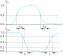
\includegraphics[scale=1]{imgBook/propagation_delay_rise_fall.pdf}
    }
    \end{textblock}
    \begin{textblock}{80}(82,70)
    \uncover<4->{
    \small
    \textcolor{verdeuca}{Físicamente las señales no son perfectas,\\ respetan un modelo de comportamiento \textbf{no lineal}}
    }
    \end{textblock}
\end{frame}

\begin{frame}[fragile,t]
    \frametitle{Retardos entre el \emph{Input} y el \emph{Output}}
    En lo que sigue vamos a simplificar el modelo, \textcolor{verdeuca}{considerando un comportamiento lineal.}
    \begin{textblock}{140}(30,22) \includegraphics[scale=1]{img/circuito_retardo-layer1.pdf} \end{textblock}
    \begin{textblock}{140}(90,22) \includegraphics[scale=1]{img/circuito_retardo-layer2.pdf} \end{textblock}
    \begin{textblock}{140}(10,50)
    \uncover<2->{
    \begin{itemize}
     \item \textbf{Propagation delay} ($\text{t}_{\text{pd}}$): Retardo hasta que el cambio de \texttt{S} termina.
     \item \textbf{Contamination delay} ($\text{t}_{\text{cd}}$): Retardo desde que \texttt{S} comienza a cambiar.
    \end{itemize}
    }
    \end{textblock}
    \begin{textblock}{140}(10,68)
    \uncover<3->{
    \textcolor{verdeuca}{Vamos a tener que calcular los caminos en el circuito, tanto el más corto, como el más largo.}
    }
    \end{textblock}
\end{frame}

\begin{frame}[fragile,t]
    \frametitle{Calculo del mayor y menor camino}
    \begin{textblock}{140}(10,12)
    Nos interesa conocer el mayor (\textcolor{naranjauca}{longest delay}) y menor (\textcolor{naranjauca}{shortest delay}) retardo en el camino dentro del circuito.
    \end{textblock}
    \begin{textblock}{140}(40,20)
    \begin{itemize}
    \item \textcolor{naranjauca}{Critical Path}: Camino más largo ($\text{t}_{\text{pd}}$)
    \item \textcolor{naranjauca}{Short Path}: Camino más corto ($\text{t}_{\text{cd}}$)
    \end{itemize}
    \end{textblock}
    \begin{textblock}{50}(13,35) \uncover<2->{\textcolor{gray}{Ejemplo:}} \end{textblock}
    \begin{textblock}{50}(13,42) \uncover<2->{\includegraphics[scale=1]{img/circuito_camino_largo_corto-layer1.pdf}} \end{textblock}
    \begin{textblock}{50}(13,42) \uncover<2->{\includegraphics[scale=1]{img/circuito_camino_largo_corto-layer2.pdf}} \end{textblock}
    \begin{textblock}{50}(13,42) \uncover<2->{\includegraphics[scale=1]{img/circuito_camino_largo_corto-layer3.pdf}} \end{textblock}
    \begin{textblock}{140}(80,45)
    \uncover<2->{
    \textcolor{naranjauca}{Critical Path}\\
    \hspace{1cm}$\text{t}_{\text{pd}}$ $=$ $2 \cdot \text{t}_{\text{pd}_{and}} + \text{t}_{\text{pd}_{or}}$\\
    \vspace{0.3cm}
    \textcolor{naranjauca}{Short Path}\\
    \hspace{1cm}$\text{t}_{\text{cd}}$ $=$ $\text{t}_{\text{cd}_{and}}$
    }
    \end{textblock}
    \begin{textblock}{140}(10,75)
    \begin{center}
    \uncover<3->{
    \textcolor{verdeuca}{El retardo de cada componente se toma de la \textbf{libreria de celdas} utilizada.}
    }
    \end{center}
    \end{textblock}
\end{frame}

\begin{frame}[fragile,t]
    \frametitle{Ejemplo de \emph{datasheet}}
    \begin{textblock}{140}(5,10)
    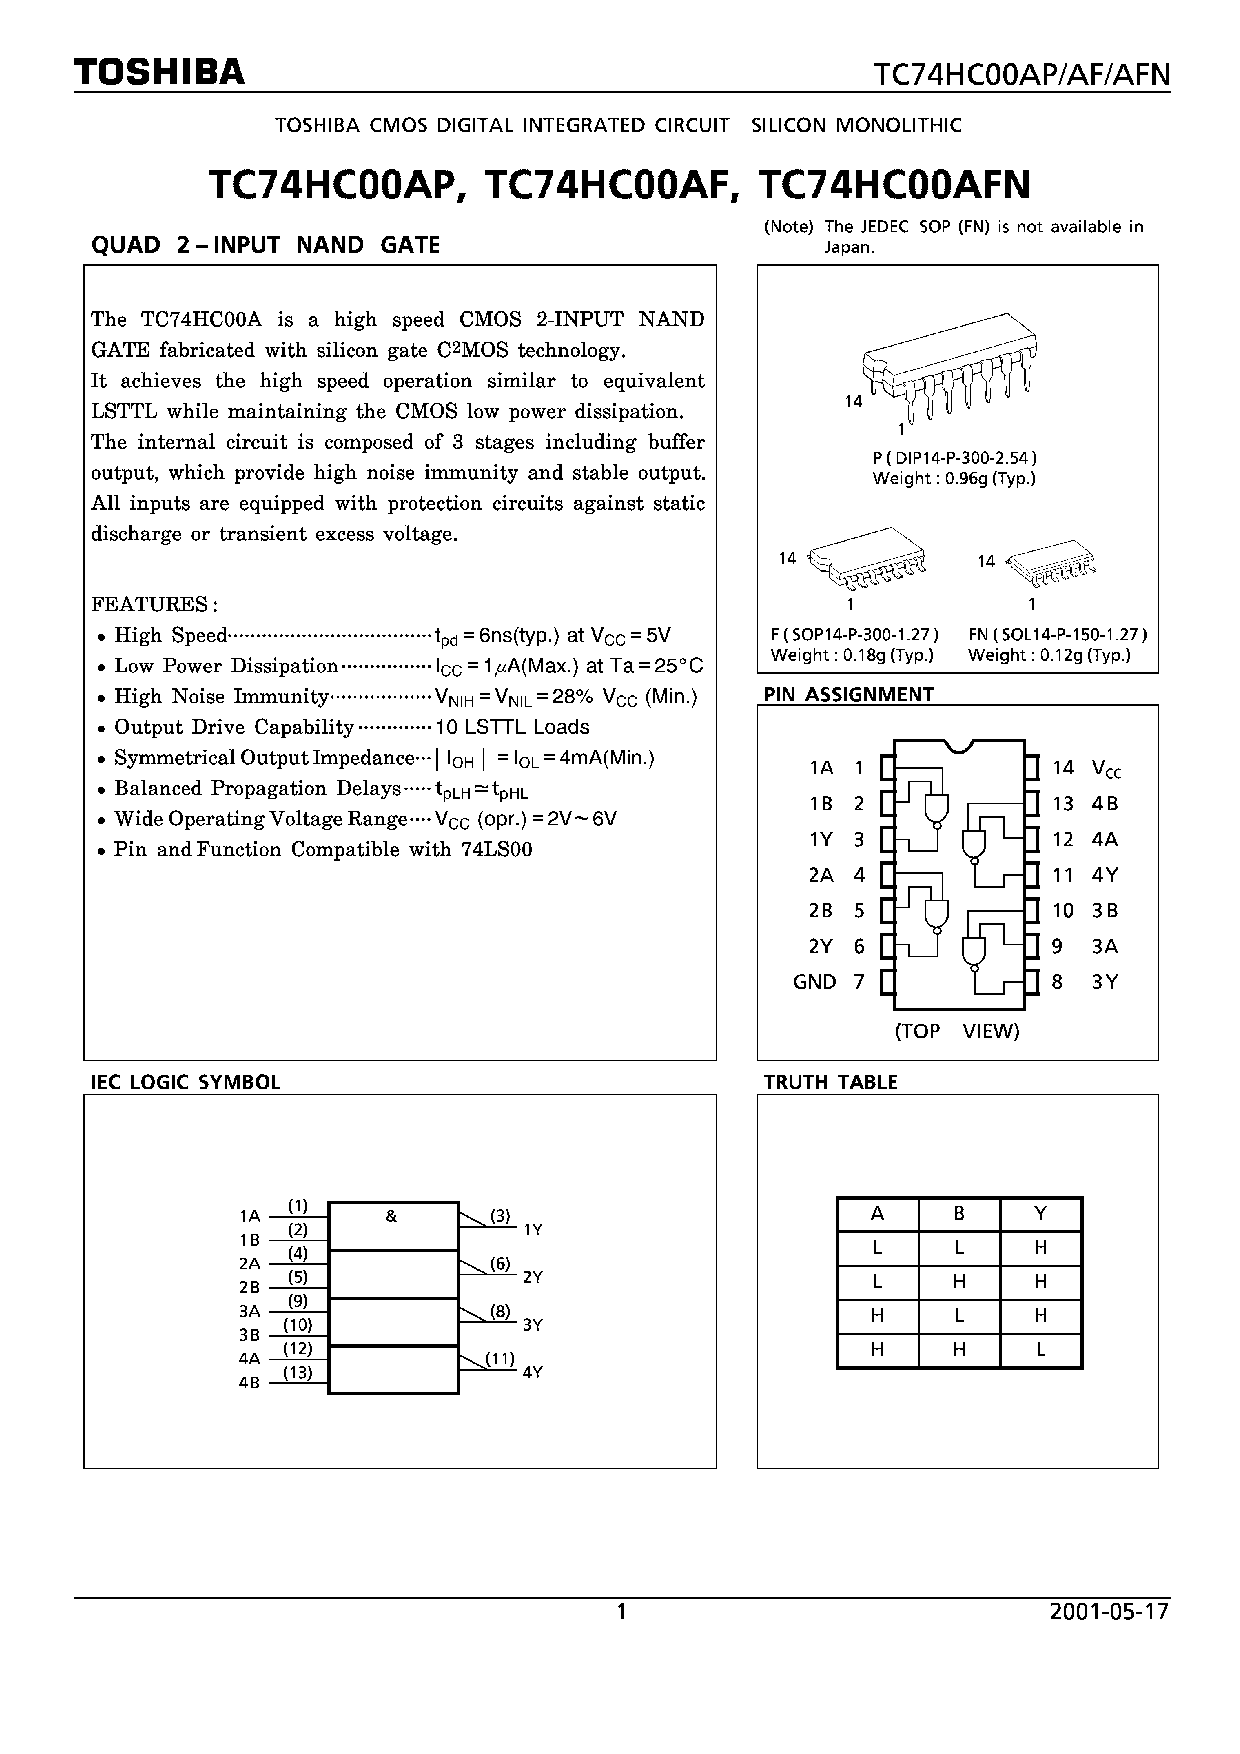
\includegraphics[page=1,trim = 0mm 116mm 0mm 0mm,clip,scale=0.37]{pdfs/TC74HC00AP.pdf}
    \end{textblock}
    \begin{textblock}{140}(80,10)
    \includegraphics[page=3,trim = 0mm 116mm 0mm 0mm,clip,scale=0.37]{pdfs/TC74HC00AP.pdf}
    \end{textblock}
\end{frame}

\begin{frame}[fragile,t]
    \frametitle{Ejemplo: Implementaciones de un multiplexor}
    \begin{textblock}{140}(10,13)
    Supongamos las siguientes implementaciones de un multiplexor y sus posibles delays.
    \end{textblock}
    \begin{textblock}{50}(10,22)
    \uncover<1->{
    \textcolor{naranjauca}{Implementación 1}\\
    \vspace{0.2cm}
    \includegraphics[scale=0.7]{img/mux2_implementaciones-layer1.pdf}\\}
    \uncover<2->{ $\text{t}_{\text{pd}}$ $=$ $\text{t}_{\text{pd}_{not}} + \text{t}_{\text{pd}_{and3}} + \text{t}_{\text{pd}_{or4}}$\\ }
    \uncover<3->{ $\text{t}_{\text{cd}}$ $=$ $\text{t}_{\text{cd}_{and3}} + \text{t}_{\text{cd}_{or4}}$}
    \end{textblock}
    \begin{textblock}{50}(60,22)
    \uncover<4->{ 
    \textcolor{naranjauca}{Implementación 2}\\
    \vspace{0.2cm}
    \includegraphics[scale=0.7]{img/mux2_implementaciones-layer2.pdf}\\}
    \uncover<5->{ $\text{t}_{\text{pd}}$ $=$ $\text{t}_{\text{pd}_{not}} + \text{t}_{\text{pd}_{and2}} + \text{t}_{\text{pd}_{buffSel}}$\\}
    \uncover<5->{ $\text{t}_{\text{cd}}$ $=$ $\text{t}_{\text{cd}_{buff}}$}
    \end{textblock}
    \begin{textblock}{50}(110,22)
    \uncover<6->{ 
    \textcolor{naranjauca}{Implementación 3}\\
    \vspace{0.2cm}
    \includegraphics[scale=0.7]{img/mux2_implementaciones-layer3.pdf}\\}
    \uncover<6->{ $\text{t}_{\text{pd}}$ $=$ $\text{t}_{\text{pd}_{buffSel}} + \text{t}_{\text{pd}_{buff}}$\\}
    \uncover<6->{ $\text{t}_{\text{cd}}$ $=$ $\text{t}_{\text{cd}_{buff}} + \text{t}_{\text{cd}_{buff}}$}
    \end{textblock}
    \begin{textblock}{140}(10,77)
    \begin{center}
    \uncover<7->{ \small \textcolor{verdeuca}{Estamos ignorando los \textbf{delay de los cables}, pero para altas frecuencias los deberíamos considerar.}}
    \end{center}
    \end{textblock}
\end{frame}

\begin{frame}[fragile,t]
    \frametitle{Ejemplo: Implementaciones de un multiplexor}
    \begin{textblock}{140}(10,13)
    Analizando las implementaciones de un multiplexor y sus posibles delays obtenemos:
    \end{textblock}
    \begin{textblock}{50}(10,22)
    \textcolor{naranjauca}{Implementación 1}\\
    $\text{t}_{\text{pd}}$ $=$ $\text{t}_{\text{pd}_{not}} + \text{t}_{\text{pd}_{and3}} + \text{t}_{\text{pd}_{or4}}$\\
    $\text{t}_{\text{pd}}$ $=$ $30 + 80 + 90$ $=$ $200$ ns\\
    \vspace{0.5cm}
    \textcolor{naranjauca}{Implementación 2}\\
    $\text{t}_{\text{pd}}$ $=$ $\text{t}_{\text{pd}_{not}} + \text{t}_{\text{pd}_{and2}} + \text{t}_{\text{pd}_{buffSel}}$\\
    $\text{t}_{\text{pd}}$ $=$ $30 + 60 + 50$ $=$ $140$ ns\\
    \vspace{0.5cm}
    \textcolor{naranjauca}{Implementación 3}\\
    $\text{t}_{\text{pd}}$ $=$ $\text{t}_{\text{pd}_{buffSel}} + \text{t}_{\text{pd}_{buff}}$\\
    $\text{t}_{\text{pd}}$ $=$ $50 + 40$ $=$ $90$ ns\\
    \end{textblock}
    \begin{textblock}{40}(90,22)
    \small \textcolor{gray}{Suponiendo los siguientes retardos para las compuertas.}\\
    \vspace{.3cm}
    \begin{tabular}{|l|c|}
    \hline
    Compuerta & $\text{t}_{\text{pd}}$ \\
    \hline
    \texttt{not}        & 30 ns \\
    \texttt{and2}       & 60 ns \\
    \texttt{and3}       & 80 ns \\
    \texttt{or4}        & 90 ns \\
    \texttt{buffSel}    & 50 ns \\
    \texttt{buff}       & 40 ns \\
    \texttt{buffNegSel} & 40 ns \\
    \texttt{buffNeg}    & 30 ns \\
    \hline
    \end{tabular}
    \end{textblock}
\end{frame}

\begin{frame}[fragile,t]
    \frametitle{Calcular \emph{long and short paths}}
    \textcolor{verdeuca}{No es simple determinar los caminos de máximos y mínimos retardos.}\\
    \begin{itemize}
    \item No todas las \textbf{entradas afectan las salidas}.
    \item Pueden existir \textbf{múltiples caminos} desde una entrada a una salida.
    \end{itemize}
    \pause
    \bigskip
    \textcolor{verdeuca}{No todos los circuitos son construidos de la misma forma.}\\
    \begin{itemize}
    \item Diferentes instancias de la misma compuerta pueden tener \textbf{diferentes retardos}.
    \item Los \textbf{cables no tiene retardo cero}, el retardo es proporcional a su longitud.
    \item La \textbf{temperatura} y el \textbf{voltaje} afecta la velocidad de los circuitos
    \begin{itemize}
    \item \textcolor{gray}{No todos los elementos en el circuito se afectan de la misma forma.}
    \item \textcolor{gray}{Incluso el \emph{critical path} puede variar dependiendo de estos factores.}
    \end{itemize}
    \end{itemize}
    \pause
    \begin{center}
    \textcolor{naranjauca}{
    Los diseñadores asumen las \textbf{peores condiciones} y terminan ejecutando muchas\\
    simulaciones para balancear una solución \textbf{conservadora} vs de \textbf{alta performance}.}
    \end{center}
\end{frame}

\begin{frame}[fragile,t]
    \frametitle{\emph{Glitches} en las salidas}
    \textcolor{naranjauca}{\emph{\textbf{glitch}}}: Un cambio en una entrada produce múltiples transiciones a la salida.\\
    \begin{textblock}{50}(13,20) \textcolor{gray}{\small  Ejemplo: Cambio en B} \end{textblock}
    \begin{textblock}{50}(13,27) \uncover<1->{\includegraphics[scale=0.9]{img/circuito_glitch-layer1.pdf}} \end{textblock}
    \begin{textblock}{50}(13,27) \uncover<3->{\includegraphics[scale=.9]{img/circuito_glitch-layer2.pdf}} \end{textblock}
    \begin{textblock}{50}(13,27) \uncover<2->{\includegraphics[scale=.9]{img/circuito_glitch-layer3.pdf}} \end{textblock}
    \begin{textblock}{50}(90,20) \uncover<1->{\includegraphics[scale=.9]{img/tiempos_glitch-layer1.pdf}} \end{textblock}
    \begin{textblock}{50}(90,20) \uncover<2->{\includegraphics[scale=.9]{img/tiempos_glitch-layer2.pdf}} \end{textblock}
    \begin{textblock}{50}(90,20) \uncover<3->{\includegraphics[scale=.9]{img/tiempos_glitch-layer3.pdf}} \end{textblock}
    \begin{textblock}{50}(90,20) \uncover<4->{\includegraphics[scale=.9]{img/tiempos_glitch-layer4.pdf}} \end{textblock}
    \begin{textblock}{140}(10,50) \uncover<4>{ \textcolor{red}{\small ¡Aparecen dos caminos, uno rápido y otro lento!} } \end{textblock}
    \begin{textblock}{140}(10,58) \uncover<4>{ 
    Los \emph{glitches} no son importantes si se diseñan correctamente los circuitos.\\ 
    \textcolor{verdeuca}{Excepto que se trabaje a frecuencias muy altas.}\\
    \bigskip
    \small \textcolor{gray}{El problema se manifiesta cuando se toma una lectura del estado del circuito en el momento de glitch.\\
    Mientras estemos seguros de diseñar el circuito y que eso nunca suceda, entonces el \emph{glitch} no debería ser un problema.}}
    \end{textblock}
\end{frame}

\begin{frame}[fragile,t]
    \frametitle{Como evitar los \emph{glitches}}
    La idea básica es utilizar \textcolor{naranjauca}{\textbf{circuitos redundantes}} que impidan que se generen los \emph{glitches},\\
    \textcolor{verdeuca}{logrando evitar que el camino más rápido haga cambiar la salida antes de tiempo.}\\
    \bigskip
    \pause
    Sin embargo, los circuitos redundantes:
    \begin{itemize}
    \item Aumentan los \textbf{costos} de diseño.
    \item Aumentan el \textbf{área}.
    \item Requieren más \textbf{energía}.
    \item Además \textbf{no (necesariamente) mejoran} el desempeño del circuito.
    \end{itemize}
    \bigskip
    \pause
    En general el diseñador debe decidir si ignorar los \emph{glitches}, \textcolor{naranjauca}{y los ignora.}
    \bigskip
    \begin{center}
    \textcolor{verdeuca}{
    En cualquier caso es necesario tenerlos en cuenta en las \textbf{simulaciones},\\
    para entender que pueden suceder y que no representan un problema.}
    \end{center}
\end{frame}

\begin{frame}[fragile,t]
    \frametitle{Timming en circuitos secuenciales}
    Para analizar la temporización de circuitos secuenciales, vamos a tomar uno\\ de los elementos que nos permite \textbf{almacenar datos}.\\
    \bigskip
    \textcolor{verdeuca}{Un Flip-flop D es circuito secuencial básico.\\
    Guarda el valor de un bit leyendolo de su entrada \texttt{D} y exponiendolo en su salida \texttt{Q}.\\
    Su activación es por el cambio de flanco en la señal de reloj.\\}
    \begin{textblock}{65}(15,48)
    \begin{center}
    \includegraphics[scale=1]{img/ff_d-layer1.pdf}
    \end{center}
    \end{textblock}
    \begin{textblock}{65}(75,48)
    \begin{tabular}{c|c|c||c}
    clk & D & Q$_\text{n}$ & Q$_\text{n+1}$ \\
       &   &              & $\textifsym{h|l}$ \\ \hline
    1  & 0 & Q$_\text{n}$ & 0 \\
    1  & 1 & Q$_\text{n}$ & 1 \\
    0  & $\times$ & Q$_\text{n}$ & Q$_\text{n}$ \\  
    \end{tabular}
    \end{textblock}
\end{frame}

\begin{frame}[fragile,t]
    \frametitle{Tiempos en un Flip-flop D (\emph{input})}
    La entrada \texttt{D} debe ser \textbf{estable} en el momento que es leída para ser copiada en el estado del circuito (activación por flanco).
    \begin{textblock}{65}(30,25)
    \includegraphics[scale=1.2]{img/ff_d-layer2.pdf}
    \end{textblock}

    \begin{textblock}{65}(78,24) \uncover<2->{\includegraphics[scale=1]{img/ff_d_tiempos-layer1.pdf}} \end{textblock}
    \begin{textblock}{65}(78,24) \uncover<3->{\includegraphics[scale=1]{img/ff_d_tiempos-layer2.pdf}} \end{textblock}
    \begin{textblock}{65}(78,24) \uncover<4->{\includegraphics[scale=1]{img/ff_d_tiempos-layer3.pdf}} \end{textblock}
    
    \begin{textblock}{140}(10,50)
    \uncover<4->{
    \textcolor{naranjauca}{\textbf{Setup time}} ($\text{t}_{\text{setup}}$):\\
    \hspace{0.5cm} Tiempo antes del cambio de flanco, donde el dato de entrada debe ser estable.\\
    \vspace{0.2cm}
    \textcolor{naranjauca}{\textbf{Hold time}} ($\text{t}_{\text{hold}}$):\\
    \hspace{0.5cm} Tiempo luego del cambio de flanco, donde el dato debe ser estable.\\
    \vspace{0.2cm}
    \textcolor{naranjauca}{\textbf{Aperture time}} ($\text{t}_{\text{a}}$):\\
    \hspace{0.5cm} Tiempo durante el cambio de flanco, donde el dato debe ser estable ($\text{t}_{\text{setup}} + \text{t}_{\text{hold}}$).\\
    }
    \end{textblock}
\end{frame}

\begin{frame}[fragile,t]
    \frametitle{Metaestabilidad: ¿Qué sucede si no respetamos los tiempos?}
    Si se violan los tiempos mínimos: \textbf{La entrada \texttt{D} cambia durante el tiempo de apertura.}\\
    \bigskip
    \pause
    Se genera {\Large \textcolor{red}{\emph{metaestability}}.}\\
    \begin{center}
    \includegraphics[scale=1.2]{img/ff_d-layer2.pdf} \hspace{2cm} 
\includegraphics[scale=1.7]{img/metaestabilidad.pdf}
    \end{center}
    La salida \texttt{Q} toma un valor entre $0$ y $1$ durante un tiempo antes de tomar el valor definitivo.\\
    \bigskip
    \pause
    El resultado será no determinístico. Puede quedar tanto en $0$ como en $1$.\\
    \begin{center}
    \textcolor{verdeuca}{La temporización de los circuitos se diseña para\\
    jamas entrar en un escenario de metaestabilidad}
    \end{center}
\end{frame}

\begin{frame}[fragile,t]
    \frametitle{Tiempos en un Flip-flop D (\emph{output})}
    La salida \texttt{Q} tomará su \textbf{valor final} luego de un tiempo dado, y comenzará a variar desde un tiempo antes.
    \begin{textblock}{65}(30,25)
    \includegraphics[scale=1.2]{img/ff_d-layer2.pdf}
    \end{textblock}
    \begin{textblock}{65}(78,20) \uncover<1->{\includegraphics[scale=1]{img/ff_d_tiempos-layer1.pdf}} \end{textblock}
    \begin{textblock}{65}(78,20) \uncover<1->{\includegraphics[scale=1]{img/ff_d_tiempos-layer2.pdf}} \end{textblock}
    \begin{textblock}{65}(78,20) \uncover<1->{\includegraphics[scale=1]{img/ff_d_tiempos-layer3.pdf}} \end{textblock}
    \begin{textblock}{65}(78,20) \uncover<2->{\includegraphics[scale=1]{img/ff_d_tiempos-layer4.pdf}} \end{textblock}
    \begin{textblock}{140}(10,63)
    \uncover<2->{
    \textcolor{naranjauca}{\textbf{Contamination delay clock-to-q}} ($\text{t}_{\text{ccq}}$):\\
    \hspace{0.5cm} Tiempo entre el cambio de flanco y que \texttt{Q} comienza a cambiar (inestable).\\
    \vspace{0.2cm}
    \textcolor{naranjauca}{\textbf{Propagacion delay clock-to-q}} ($\text{t}_{\text{pcq}}$):\\
    \hspace{0.5cm} Tiempo entre el cambio de flanco y que \texttt{Q} deja de cambiar (estable).
    }
    \end{textblock}
\end{frame}

\begin{frame}[fragile,t]
    \frametitle{Temporización de sistemas secuenciales}
    Un sistema secuencial se puede ver como \textbf{múltiples flip-flops interconectados}\\
    mediante circuitos combinatorios puros.
    \begin{center}
     
\includegraphics[scale=1]{img/sistema_secuencial.pdf}
    \end{center}
    \pause
    Para asegurar el correcto funcionamiento debemos verificar que se cumplen\\
    los \textbf{requerimientos de tiempo}, tanto para \texttt{F$_\text{n}$} como para \texttt{F$_{\text{n+1}}$}.\\
    \bigskip
    \pause
    \textcolor{verdeuca}{Para asegurar que \texttt{F$_{\text{n+1}}$} tome el valor correcto}:\\
    \texttt{D$_{\text{n+1}}$}, debe ser \textbf{estable} durante el tiempo de apertura de \texttt{F$_{\text{n+1}}$}.\\
    \begin{itemize}
    \item Si la lógica combinacional es \textcolor{naranjauca}{\textbf{muy rápida}}, entonces el \textcolor{naranjauca}{\textbf{\emph{hold time} no se cumple}}.
    \item Si la lógica combinacional es \textcolor{naranjauca}{\textbf{muy lenta}}, entonces  el \textcolor{naranjauca}{\textbf{\emph{setup time} no se cumple}}.
    \end{itemize}
\end{frame}

\begin{frame}[fragile,t]
    \frametitle{Limitaciones del tiempo de \emph{setup}} % \emph{Safe timming}: 
    Para asegurar el tiempo se debe \textbf{limitar el retardo máximo} entre \texttt{F$_\text{n}$} y \texttt{F$_{\text{n+1}}$}.\\
    La entrada de \texttt{F$_{\text{n+1}}$} debe ser \textbf{estable} al menos $\text{t}_{\text{setup}}$ antes del cambio de clock.
    \begin{textblock}{100}(10,23)
    \uncover<2->{ 
\includegraphics[scale=1]{img/sistema_secuencial.pdf} }
    \end{textblock}
    \begin{textblock}{100}(80,23)
    \uncover<2->{ \includegraphics[scale=1]{img/tiempos_seguros-layer1.pdf} }
    \end{textblock}
    \begin{textblock}{60}(10,43)
    \begin{center}
    \uncover<3->{ {\Large $\text{T}_\text{c}$ $>$ $\text{t}_{\text{pcq}} + \text{t}_{\text{pd}} + \text{t}_{\text{setup}}$}\\ }
    \end{center}
    \end{textblock}
    \begin{textblock}{100}(10,60)
    \uncover<3->{ 
    Donde,\\
    \hspace{0.5cm} $\text{T}_\text{c}$ $\rightarrow$ \textcolor{verdeuca}{Tiempo del ciclo de reloj.}\\
    \hspace{0.5cm} $\text{t}_{\text{pd}}$ $\rightarrow$ \textcolor{verdeuca}{Tiempo útil del circuito.}\\
    \hspace{0.5cm} $\text{t}_{\text{pcq}}$ $\rightarrow$ \textcolor{verdeuca}{Tiempo perdido para escribir el próximo dato.}\\
    \hspace{0.5cm} $\text{t}_{\text{setup}}$ $\rightarrow$ \textcolor{verdeuca}{Tiempo perdido para leer el próximo dato.}\\
    }
    \end{textblock}
    \begin{textblock}{40}(105,65)
    \uncover<4->{
    \small
    El tiempo desperdiciado en garantizar la secuencialidad de los eventos se denomina \textcolor{naranjauca}{\textbf{Secuencial Overhead}}.\\
    ($\text{t}_{\text{pcq}} + \text{t}_{\text{setup}}$)
    }
    \end{textblock}
\end{frame}

\begin{frame}[fragile,t]
    \frametitle{Limitaciones del tiempo de \emph{setup}} % \emph{Safe timming}: 
    \begin{textblock}{100}(10,15)
    
\includegraphics[scale=1]{img/sistema_secuencial.pdf}       
    \end{textblock}
    \begin{textblock}{100}(80,15)
    \includegraphics[scale=1]{img/tiempos_seguros-layer1.pdf}
    \end{textblock}
    \begin{textblock}{60}(10,38)
    \begin{center}
    {\Large $\text{T}_\text{c}$ $>$ $\text{t}_{\text{pcq}} + \text{t}_{\text{pd}} + \text{t}_{\text{setup}}$}\\
    \end{center}
    \end{textblock}
    \begin{textblock}{140}(10,60)
    El rendimiento del diseño está determinado por el \emph{critical path} ($\text{t}_{\text{pd}}$).\\
    \uncover<2->{ Este permite determinar el mínimo \emph{clock period}, o \textcolor{naranjauca}{\textbf{frecuencia máxima}} de operación.}
    \uncover<2->{ 
    \begin{itemize}
    \item \textcolor{verdeuca}{Si el \emph{critical path} es muy \textbf{grande}, el diseño resulta \textbf{muy lento}.}
    \item \textcolor{verdeuca}{Si el \emph{critical path} es muy \textbf{chico}, en cada ciclo estamos haciendo \textbf{poco trabajo útil}}\\
    \textcolor{verdeuca}{\small (la mayor parte del ciclo se pierde en el secuencial overhead).}
    \end{itemize}
    }
    \end{textblock}
\end{frame}

\begin{frame}[fragile,t]
    \frametitle{Limitaciones del tiempo de \emph{hold}} % \emph{Safe timming}: 
    Para asegurar el tiempo se debe \textbf{limitar el retardo mínimo} entre \texttt{F$_\text{n}$} y \texttt{F$_{\text{n+1}}$}\\
    $\text{D}_{\text{n+1}}$ debe ser \textbf{estable} al menos $\text{t}_{\text{hold}}$ luego del cambio de clok.
    \begin{textblock}{100}(10,23)
    \uncover<2->{ 
\includegraphics[scale=1]{img/sistema_secuencial.pdf} }
    \end{textblock}
    \begin{textblock}{100}(80,23)
    \uncover<2->{ \includegraphics[scale=1]{img/tiempos_seguros-layer2.pdf} }
    \end{textblock}
    \begin{textblock}{60}(10,43)
    \begin{center}
    \uncover<3->{ {\Large $\text{t}_{\text{ccq}} + \text{t}_{\text{cd}}$ $>$ $\text{t}_{\text{hold}}$}\\
    o\\
    {\Large $\text{t}_{\text{cd}}$ $>$ $\text{t}_{\text{hold}} - \text{t}_{\text{ccq}}$}\\ }
    \end{center}
    \end{textblock}
    \begin{textblock}{140}(10,67)
    \uncover<3->{   
    El \emph{contamination delay} ($\text{t}_{\text{cd}}$) del circuito combinacional no puede ser cero,\\
    debe tener un mínimo de tiempo de al menos $\text{t}_{\text{hold}} - \text{t}_{\text{ccq}}$.\\
    }
    \bigskip
    \uncover<4->{ 
    \textbf{No depende del reloj ($\text{T}_\text{c}$), depende del \textcolor{red}{diseño del circuito}.}
    }
    \end{textblock}
\end{frame}

\begin{frame}[fragile,t]
    \frametitle{Ejemplo de análisis de tiempo}
    
    \begin{textblock}{140}(5,12) \uncover<1->{ \includegraphics[scale=1]{img/circuito_ejemplo_tiempos-layer1.pdf}} \end{textblock}
    \begin{textblock}{140}(5,12) \uncover<3->{ \includegraphics[scale=1]{img/circuito_ejemplo_tiempos-layer2.pdf}} \end{textblock}
    \begin{textblock}{140}(5,12) \uncover<4->{ \includegraphics[scale=1]{img/circuito_ejemplo_tiempos-layer3.pdf}} \end{textblock}

    \begin{textblock}{50}(10,50)
    \uncover<2->{ 
    \begin{tabular}{l|l}
    Valor    & Tiempo \\ \hline
    $\text{t}_\text{ccq}$   & 30 ps \\
    $\text{t}_\text{pcq}$   & 50 ps \\
    $\text{t}_\text{setup}$ & 60 ps \\
    $\text{t}_\text{hold}$  & 70 ps \\
    $\text{t}_\text{pd}$    & 35 ps (all gates) \\
    $\text{t}_\text{cd}$    & 25 ps (all gates) \\
    \end{tabular}
    }
    \end{textblock}

    \begin{textblock}{60}(85,8)
    \uncover<3->{ $\text{t}_\text{pd}$ $=$ $35 + 35 + 35$ ps $=$ $105$ ps\\ }
    \uncover<4->{ $\text{t}_\text{cd}$ $=$ $25$ ps\\ }
    \bigskip
    \uncover<5->{
    Validación \emph{setup time}:\\
    {$\text{T}_\text{c}$ $>$ $\text{t}_{\text{pcq}} + \text{t}_{\text{pd}} + \text{t}_{\text{setup}}$}\\    
    {$\text{T}_\text{c}$ $>$ $50 + 105 + 60$}\\
    {$\text{T}_\text{c}$ $>$ $215$}\\
    {$\text{Frec}_\text{max}$ $=$ $1/\text{T}_\text{c}$ $=$ $4.65$ GHz}\\
    }
    \bigskip
    \uncover<6->{
    Validación \emph{hold time}:\\
    {$\text{t}_{\text{ccq}} + \text{t}_{\text{cd}}$ $>$ $\text{t}_{\text{hold}}$}\\
    {$35 + 25$ $>$ $70$}\\
    {$55$ $>$ $70$}\\
    }
    \uncover<7->{
    \textcolor{rojo}{¡No verifica!\\}
    \bigskip
    \textcolor{rojo}{\textbf{Debemos alterar el circuito para que\\ el camino mínimo sea más largo}.}
    }
    \end{textblock}
\end{frame}


\begin{frame}[fragile,t]
    \frametitle{Ejemplo de análisis de tiempo}
    
    \begin{textblock}{140}(5,12) \includegraphics[scale=1]{img/circuito_ejemplo_tiempos-layer1.pdf} \end{textblock}
    \begin{textblock}{140}(5,12) \includegraphics[scale=1]{img/circuito_ejemplo_tiempos-layer2.pdf} \end{textblock}
    \begin{textblock}{140}(5,12) \includegraphics[scale=1]{img/circuito_ejemplo_tiempos-layer3.pdf} \end{textblock}
    \begin{textblock}{140}(5,12) \includegraphics[scale=1]{img/circuito_ejemplo_tiempos-layer4.pdf} \end{textblock}

    \begin{textblock}{50}(10,50)
    \begin{tabular}{l|l}
    Valor    & Tiempo \\ \hline
    $\text{t}_\text{ccq}$   & 30 ps \\
    $\text{t}_\text{pcq}$   & 50 ps \\
    $\text{t}_\text{setup}$ & 60 ps \\  
    $\text{t}_\text{hold}$  & 70 ps \\
    $\text{t}_\text{pd}$    & 35 ps (all gates) \\
    $\text{t}_\text{cd}$    & 25 ps (all gates) \\
    \end{tabular}
    \end{textblock}

    \begin{textblock}{50}(85,8)
    $\text{t}_\text{pd}$ $=$ $35 + 35 + 35$ ps $=$ $105$ ps\\
    $\text{t}_\text{cd}$ $=$ $25 + 25$ ps $=$ $50$ ps\\
    \bigskip
    Validación \emph{setup time}:\\
    {$\text{T}_\text{c}$ $>$ $\text{t}_{\text{pcq}} + \text{t}_{\text{pd}} + \text{t}_{\text{setup}}$}\\    
    {$\text{T}_\text{c}$ $>$ $50 + 105 + 60$}\\
    {$\text{T}_\text{c}$ $>$ $215$}\\
    {$\text{Frec}_\text{max}$ $=$ $1/\text{T}_\text{c}$ $=$ $4.65$ GHz}\\

    \bigskip
    Validación \emph{hold time}:\\
    {$\text{t}_{\text{ccq}} + \text{t}_{\text{cd}}$ $>$ $\text{t}_{\text{hold}}$}\\
    {$35 + 50$ $>$ $70$}\\
    {$85$ $>$ $70$}\\
    \textcolor{v}{¡Verifica!}

    \end{textblock}
\end{frame}

\begin{frame}[fragile,t]
    \frametitle{Clock Skew: El reloj también tiene retardo}
    La señal de reloj no llega a todos los rincones del circuito al mismo tiempo.\\
    \textcolor{verdeuca}{No todos los componentes secuenciales ven el reloj en el \textbf{mismo momento.}}\\
    \bigskip
    \textcolor{naranjauca}{\textbf{Clock Skew}}: es la diferencia entre dos cambios de flanco del mismo reloj en lugares diferentes.\\
    \bigskip
    \begin{textblock}{100}(10,36) \uncover<1->{ \includegraphics[]{img/clock_skew_path-layer1.pdf}} \end{textblock}
    \begin{textblock}{100}(10,36) \uncover<2->{ \includegraphics[]{img/clock_skew_path-layer2.pdf}} \end{textblock}
    \begin{textblock}{100}(10,36) \uncover<3->{ \includegraphics[]{img/clock_skew_path-layer3.pdf}} \end{textblock}
    \begin{textblock}{100}(10,36) \uncover<4->{ \includegraphics[]{img/clock_skew_path-layer4.pdf}} \end{textblock}
    \begin{textblock}{100}(10,36) \uncover<5->{ \includegraphics[]{img/clock_skew_path-layer5.pdf}} \end{textblock}
    \begin{textblock}{100}(100,36) \uncover<1->{ \includegraphics[]{img/clock_skew_circuito-layer1.pdf}} \end{textblock}
    \begin{textblock}{100}(100,36) \uncover<2->{ \includegraphics[]{img/clock_skew_circuito-layer2.pdf}} \end{textblock}
    \begin{textblock}{100}(100,36) \uncover<3->{ \includegraphics[]{img/clock_skew_circuito-layer3.pdf}} \end{textblock}
    \begin{textblock}{100}(100,36) \uncover<4->{ \includegraphics[]{img/clock_skew_circuito-layer4.pdf}} \end{textblock}
    \begin{textblock}{140}(10,76) \uncover<5->{ 
    \textbf{Este problema hace el calculo aun más complejo},\\
    el reloj puede llegar \textcolor{naranjauca}{antes} o \textcolor{naranjauca}{despues} que el reloj de la próxima etapa.
    } \end{textblock}
\end{frame}

\begin{frame}[fragile,t]
    \frametitle{Clock Skew: Ejemplo procesador DEC Alpha}    
    \begin{textblock}{100}(10,0) \includegraphics[scale=0.65]{img/clock_skew_gronowski.pdf} \end{textblock}
    \begin{textblock}{150}(5,86)
    \scriptsize
    ``High-Performance Microprocessor Design'' P. E. Gronowski, et. al.
    IEEE JOURNAL OF SOLID-STATE CIRCUITS, VOL. 33, NO. 5, MAY 1998
    \end{textblock}
    % DEC Alpha clock grids panels drivers
    % 21064 (1993): 200MHz 0.75μm process -> one driver pane
    % 21164 (1996): 333MHz 0.50μm process -> two driver panes
    % 21264 (1997): 600MHz 0.35μm process -> sixteen driver panes
\end{frame}

\begin{frame}[fragile,t]
    \frametitle{Clock Skew: Limitaciones del tiempo de \emph{setup}}
    Supongamos el peor caso para el \emph{Clock Skew}. \textbf{La señal de reloj llega a $\text{F}_{\text{n+1}}$ antes que a $\text{F}_{\text{n}}$.}\\
    \textcolor{verdeuca}{Esto reduce el tiempo que disponemos para resolver el circuito combinatorio.}
    \begin{textblock}{100}(10,23)
    \uncover<1->{ \includegraphics[scale=1]{img/sistema_secuencial.pdf} }
    \end{textblock}
    \begin{textblock}{100}(80,23)
    \uncover<2->{ \includegraphics[scale=1]{img/clock_skew_tiempos_seguros-layer1.pdf} }
    \end{textblock}
    \begin{textblock}{60}(10,43)
    \uncover<3->{
    \begin{center}
    {\Large $\text{T}_\text{c}$ $>$ $\text{t}_{\text{pcq}} + \text{t}_{\text{pd}} + \text{t}_{\text{setup}} + \text{t}_{\text{skew}}$}\\
    \end{center}
    }
    \end{textblock}
    \begin{textblock}{140}(10,60)
    \uncover<4->{
    Luego,\\
    {\Large $\text{t}_{\text{pd}}$ $<$ $\text{T}_\text{c} - ( \text{t}_{\text{pcq}} + \text{t}_{\text{setup}} + \text{t}_{\text{skew}} ) $}\\
    }
    \bigskip
    \uncover<5->{
    Considerando \emph{skew time}, esté se materializa como un aumento en el \emph{setup time}.\\
    \textcolor{verdeuca}{Limita aun más el tiempo de propagación máximo del circuito combinatorio ($\text{t}_{\text{pd}}$).}
    }
    \end{textblock}
\end{frame}

\begin{frame}[fragile,t]
    \frametitle{Clock Skew: Limitaciones del tiempo de \emph{hold}}
    Supongamos el peor caso para el \emph{Clock Skew}. \textbf{La señal de reloj llega a $\text{F}_{\text{n+1}}$ despues que a $\text{F}_{\text{n}}$.}\\
    \textcolor{verdeuca}{Esto incrementa el tiempo mínimo que debe tener como retardo el circuito combinatorio.}
    \begin{textblock}{100}(10,23)
    \uncover<1->{ \includegraphics[scale=1]{img/sistema_secuencial.pdf} }
    \end{textblock}
    \begin{textblock}{100}(80,23)
    \uncover<2->{ \includegraphics[scale=1]{img/clock_skew_tiempos_seguros-layer2.pdf} }
    \end{textblock}
    \begin{textblock}{60}(10,43)
    \uncover<3->{
    \begin{center}
    {\Large $\text{t}_\text{cd} + \text{t}_{\text{ccq}}$ $>$ $\text{t}_{\text{hold}} + \text{t}_{\text{skew}}$}\\
    \end{center}
    }
    \end{textblock}
    \begin{textblock}{120}(10,60)
    \uncover<4->{
    Luego,\\
    {\Large $\text{t}_\text{cd}$ $>$ $\text{t}_{\text{hold}} + \text{t}_{\text{skew}} - \text{t}_{\text{ccq}}$}\\
    }
    \bigskip
    \uncover<5->{ 
    Considerando \emph{skew time}, esté se materializa como un aumento en el \emph{hold time}.\\
    \textcolor{verdeuca}{Limita aun más el tiempo mínimo del circuito combinatorio ($\text{t}_{\text{cd}}$).}
    }
    \end{textblock}
\end{frame}

\begin{frame}[fragile,t]
    \frametitle{Clock Skew}
    El \emph{Clock Skew} incrementa los tiempos de $\text{t}_{\text{setup}}$ y $\text{t}_{\text{hold}}$.\\
    \textcolor{verdeuca}{Aumenta el \textbf{secuencial overhead}, dejando menos tiempo para el trabajo útil por ciclo de reloj.}\\
    \bigskip
    \uncover<2->{
    Se buscan reducir al\\
    mínimo el \emph{Clock Skew}.\\
    \bigskip
    \small
    \textcolor{gray}{
    Diseñando inteligentes\\
    formas de distribuir el\\
    reloj a lo largo del circuito.\\
    }
    \bigskip
    \emph{Pre-drivers}, \emph{Clock-tree},\\
    \emph{Cross-links}, \emph{Mesh}, \emph{Sinks},\\
    son algunas de las técnicas\\
    que se utilizan.\\}
    \begin{textblock}{100}(50,28)  \uncover<2->{\includegraphics[scale=0.7]{img/clock_distribution-layer1.pdf}} \end{textblock}
    \begin{textblock}{100}(85,28)  \uncover<3->{\includegraphics[scale=0.7]{img/clock_distribution-layer2.pdf}} \end{textblock}
    \begin{textblock}{100}(120,28) \uncover<4->{\includegraphics[scale=0.7]{img/clock_distribution-layer3.pdf}} \end{textblock}
\end{frame}

\begin{frame}[fragile,t]
    \frametitle{Verificación de circuitos}
    \begin{center}
    \textcolor{naranjauca}{\Large \textbf{¿Cómo sabemos que un circuito funciona correctamente?}}\\
    \bigskip
    \pause
    \textcolor{verdeuca}{Incluso si es logicamente correcto, puede que el hardware donde lo vamos a\\ implementar no pueda respetar todas las limitaciones de tiempos del diseño.}\\
    \end{center}
    \pause
    Tipos de comprobaciones:\\
    \begin{itemize}
    \item Testeo \textbf{funcional}: Respeta el comportamiento descripto por el HDL.
    \item Testeo \textbf{temporal}: Respeta las limitaciones de tiempo del hardware.
    \end{itemize}
    \bigskip
    \pause
    Herramientas de simulación:\\
    \begin{itemize}
     \item \textbf{Verificación formal}: Modelo matemático (ej. SAT solvers).
     \item \textbf{Simulación desde HDL}: Simulación de alto nivel (ej. Vivado).
     \item \textbf{Simulación del circuito}: Simulación de bajo nivel (ej. SPICE).
    \end{itemize}
\end{frame}

\begin{frame}[fragile,t]
    \frametitle{Verificación de circuitos: El problema de los diseños muy grandes}
    La verificación del diseño puede llevar mucho tiempo.\\
    \begin{itemize}
    \item Todos los \textbf{caminos lógicos} del circuito son funcionalmente correctos.
    \item Todos los \textbf{elementos del circuito} se usan dentro de los límites de tiempo y energía.
    \end{itemize}
    \pause
    \bigskip
    La comprobación entonces se separa en dos responsabilidades:\\
    \vspace{0.2cm}
    \begin{enumerate}
    \setlength\itemsep{0.2cm}
    \item<2-> \textbf{Chequeo solo de la \textcolor{naranjauca}{funcionalidad a alto nivel}, sobre el circuito desde el HDL.}
    \begin{itemize}
    \item \textcolor{verdeuca}{Más rápido que a nivel de circuitos, permite \textbf{cubrir mayor cantidad de posibilidades}.}
    \item \textcolor{verdeuca}{\textbf{Fácil de escribir} y correr comprobaciones.}
    \end{itemize}
    \item<3-> \textbf{Chequeo solo de \textcolor{naranjauca}{tiempo, energía y límites a bajo nivel}, sobre el circuito.}
    \begin{itemize}
    \item \textcolor{verdeuca}{\textbf{No se realiza un chequeo funcional} del modelo a bajo nivel.}
    \item \textcolor{verdeuca}{Se chequea un \textbf{modelo funcional equivalente} al de alto nivel, que resulta más simple que comprobar el funcionamiento completo a este nivel.}
    \end{itemize}
    \end{enumerate}
    \vspace{0.2cm}
    \uncover<3->{
    La simulación del circuito (bajo nivel) es más lenta que la simulación desde HDL (alto nivel).}
\end{frame}

\begin{frame}[fragile,t]
    \frametitle{Verificación de circuitos: El problema de los diseños muy grandes}
    Tenemos herramientas para manejar \textbf{diferentes niveles de verificación}.\\
    \begin{itemize}
    \item<2-> \textcolor{naranjauca}{\textbf{Logical Syntesis tools}}: Comprobar equivalencia entre la lógica de alto nivel y la sintetización a nivel de descripción del circuito.
    \item<3-> \textcolor{naranjauca}{\textbf{Timming verification tools}}: Comprobar la temporización del circuito en base a una tecnología de implementación.  
    \item<4-> \textcolor{naranjauca}{\textbf{Design rule checks}}: Comprobar que la implementación del circuito sea físicamente realizable.
    \end{itemize}
    \bigskip
    \uncover<5->{
    El objetivo del diseñador de la lógica del circuito es:
    \begin{itemize}
    \item Proveer \textbf{test funcionales} para comprobar la correctitud del diseño.
    \item Proveer \textbf{timing contraints}, por ejemplo, la deseable frecuencia de operación.
    \end{itemize}
    \bigskip
    \textcolor{verdeuca}{Los ingenieros de circuitos usando estas herramientas deciden si el diseño se puede construir.}
    }
\end{frame}

\begin{frame}[fragile,t]
    \frametitle{Verificación Funcional }
    Consiste en un chequeo \emph{booleano}. Se busca comprobar la correctitud encontrando un contraejemplo para su correcto funcionamiento.\\
    \bigskip
    \begin{center}
    {\Large \textcolor{red}{Objetivo:} Chequeo de la correctitud lógica del diseño}
    \end{center}
    \bigskip
    \pause
    En este caso la \textbf{temporización es ignorada}.\\
    \textcolor{verdeuca}{Sin embargo, se comprueban chequeos simples para encontrar problemas básicos.}\\
    \bigskip
    \pause
    Dos enfoques principales:
    \begin{itemize}
    \item Simulación lógica (\textit{rutinas de test}). $\rightarrow$ \textcolor{naranjauca}{¡esto es lo que vamos a hacer!}
    \item Técnicas de verificación formal.
    \end{itemize}
\end{frame}

\begin{frame}[fragile,t]
    \frametitle{Verificación funcional basada en \emph{Testbench}}
    Un \emph{Testbench} es un módulo de Verilog creado específicamente para testear un diseño.\\
    Usualmente llamado ``device under test (DUT)''\\
    \begin{center}
    \includegraphics[scale=0.8]{img/testbench.pdf}
    \end{center}
    \pause
    Un \emph{Testbench} provee \textbf{entradas} (patrones) al DUT.
    \begin{itemize}
    \item Generados manualmente.
    \item Generados automáticamente (secuencial o aleatorios).
    \end{itemize}
    \bigskip
    \pause
    Un \emph{Testbench} chequea las \textbf{salidas} del DUT contra las correctas.
    \begin{itemize}
    \item Validadas manualmente.
    \item Validadas contra un modelo libre de errores (\emph{``golden design''}).
    \end{itemize}
\end{frame}

\begin{frame}[fragile,t]
    \frametitle{Verificación funcional basada en Testbench}
    \textcolor{verdeuca}{Un \emph{Testbench} puede ser:}
    \begin{itemize}
    \item \textbf{Código HDL} escrito para testear otros modulos HDL.
    \item \textbf{Circuito esquemático} usado para testear otros diseños.
    \end{itemize}
    \pause
    \textcolor{verdeuca}{Un \emph{Testbench} no esta diseñado para sintetizar en hardware:}
    \begin{itemize}
    \item<3-> Ejecuta \textbf{solo en una simulación}.
    \begin{itemize}
    \item Simulación HDL (Vivado Simulator).
    \item Simulación del circuito (SIPICE).
    \end{itemize}
    \item<4-> Usa herramientas \textbf{válidas solo dentro de la simulación}.
    \begin{itemize}
    \item Marcas de espera por un tiempo fijo.
    \item Indicaciones de voltajes y corrientes ideales.
    \item No considera la construcción física del circuito.
    \end{itemize}
    \end{itemize}
    \bigskip
    \uncover<5->{\textcolor{naranjauca}{\textbf{Tipos de Testbench}}\\}
    \vspace{5cm}
    \begin{textblock}{100}(45,65)
    \uncover<5->{
    \small
    \begin{tabular}{|c|c|c|} \hline
    \cellcolor{verdeuca} \color[HTML]{FFFFFF} Testbench    & \color[HTML]{FFFFFF} \cellcolor{verdeuca} Generación de entradas y salidas & \color[HTML]{FFFFFF} \cellcolor{verdeuca} Chequeo de errores \\  \hline
    \cellcolor[HTML]{CBCBCB} Simple       & Manual     & Manual     \\
    \cellcolor[HTML]{CBCBCB} Auto-Chequeo & Manual     & Automático \\
    \cellcolor[HTML]{CBCBCB} Automático   & Automático & Automático \\  \hline
    \end{tabular}
    }
    \end{textblock}
\end{frame}

\begin{frame}[fragile,t]
    \frametitle{Ejemplo: Testbench Simple}
    \begin{textblock}{70}(10,15)
\lstset{basicstyle=\scriptsize}
\begin{lstlisting}
module testbench_Simple();
    reg a, b, c;
    wire y;
    
    fun dut(.a(a), .b(b), .c(c), .y(y));

    initial begin
        a = 0; b = 0; c = 0;
        #10;
        c = 1;
        #10;
        b = 1; c = 0;
        #10
        a = 1; b = 0; c = 0;
        #10;
        ...
    end
endmodule
\end{lstlisting}
    \end{textblock}
    \begin{textblock}{60}(85,15)
    \small
    \uncover<1->{ Reproduce un conjunto de señales que se envían al \texttt{DUT} cada un tiempo determinado.\\ }
    \bigskip
    \uncover<2->{ La simulación registra el cambio de las señales.
    \textcolor{verdeuca}{Idealmente se utilizan diagramas de señales para visualizar los cambios.}\\ }
    \bigskip
    \uncover<3->{ \textcolor{rojo}{Para circuitos grandes, con muchas señales está solución no escala.} }
    \end{textblock}
    \begin{textblock}{140}(85,55)
    \only<3->{ 
    \includegraphics[page=1,trim = 5mm 154mm 370mm 3mm,clip,scale=0.24]{bitmap/signals.png}
    }
    \end{textblock}
\end{frame}

\begin{frame}[fragile,t]
    \frametitle{Testbench Simple}
    \textcolor{v}{\textbf{Pro:}}\\
    \begin{itemize}
    \item Simple de diseñar y hacer.
    \item Fácil testear, pocas entradas y casos borde.
    \item Útil para aprender.
    \end{itemize}
    \pause
    \textcolor{r}{\textbf{Contras:}}\\
    \begin{itemize}
    \item No escala para circuitos grandes.
    \item Las salidas deben ser chequeadas \textbf{manualmente} fuera de la simulación.
    \begin{itemize}
    \item Mirando las señales una por una.
    \item Imprimiendo en un \emph{log} de salida.
    \end{itemize}
    \end{itemize}
\end{frame}

\begin{frame}[fragile,t]
    \frametitle{Ejemplo: Testbench Auto-Chequeo}
    \begin{textblock}{75}(10,10)
\lstset{basicstyle=\scriptsize}
\begin{lstlisting}
module testbench_AutoChequeo();
    reg a, b, c;
    wire y;
    
    fun dut(.a(a), .b(b), .c(c), .y(y));

    initial begin
        a = 0; b = 0; c = 0;
        #10;
        if( y !== 1) $display("error 000");
        c = 1;
        #10;
        if( y !== 0) $display("error 001");
        b = 1; c = 0;
        #10
        if( y !== 0) $display("error 010");
        a = 1; b = 0; c = 0;
        #10;
        if( y !== 1) $display("error 100");
        ...
    end
endmodule
\end{lstlisting}
    \end{textblock}
    \begin{textblock}{55}(90,15)
    \small
    \uncover<1->{ Agregando muy poca lógica es posible hacer chequeos en el código de test.\\ }
    \bigskip
    \uncover<2->{ Los chequeos consisten en comparaciones con estados conocidos.\\ }
    \bigskip
    \uncover<3->{ \textcolor{rojo}{Para circuitos grandes, con muchos estados es muy complicado generar todos los casos de prueba y sus soluciones esperadas.} }
    \end{textblock}
\end{frame}

\begin{frame}[fragile,t]
    \frametitle{Testbench Auto-Chequeo}
    \textcolor{v}{\textbf{Pro:}}\\
    \begin{itemize}
    \item Simple de diseñar y hacer.
    \item Fácil testear pocas entradas y casos borde.
    \item El simulador indica cuando un error ocurre.
    \end{itemize}
    \pause
    \textcolor{r}{\textbf{Contras:}}\\
    \begin{itemize}
    \item No escala para circuitos grandes.
    \item Es fácil cometer un error sobre los valores fijados como válidos.
    \item El proceso de \emph{debug} es difícil, ya que se debe identificar si el error está en el test o en el \texttt{DUT}.
    \end{itemize}
\end{frame}
  
\begin{frame}[fragile,t]
    \frametitle{Testbench Auto-Chequeo usando \texttt{testvectors}}
    La idea es tener un archivo con todas las entradas y salidas a verificar.\\
    \textcolor{verdeuca}{El archivo se puede crear de forma manual o automática\\ a partir de un modelo de funcionamiento verificado.}
    \begin{textblock}{45}(10,30)
    \begin{onlyenv}<2->
    Ejemplo: \texttt{input\_output}
\begin{lstlisting}  
    000_1
    001_0
    010_1
    011_0
    100_1
    101_0
    110_1
    111_0
\end{lstlisting}
    \end{onlyenv}
    \end{textblock}
    \begin{textblock}{75}(70,30)
    \uncover<2->{
    Usando una nueva señal de reloj para asignar entradas y leer salidas.\\
    \bigskip
    Ejecutamos una a una las entradas por cada ciclo de nuestro nuevo reloj.\\}
    \small
    \uncover<3->{
    \begin{itemize}
    \item \textcolor{verdeuca}{La señal sirve para separar las entradas de la lectura de salidas.}
    \item \textcolor{verdeuca}{Permite observar en los diagramas de señales las entradas y salidas.}
    \end{itemize}
    }
    \end{textblock}
\end{frame}

\begin{frame}[fragile,t]
    \frametitle{Ejemplo: Testbench Auto-Chequeo usando \texttt{testvectors}}

    \begin{textblock}{55}(10,12)
\lstset{basicstyle=\tiny, columns=flexible, stepnumber=1, numbers=left}
\begin{lstlisting}
module testbench_AutoChequeo_TestVectors();
    reg clk, reset;
    reg a, b, c;
    wire y;
    reg [31:0] vectornum, errors;
    reg [31:0] testvector[0:1000];
    
    circuit dut(.a(a), .b(b), .c(c), .y(y));

    always @(*)
        clk = 1; #5; clk = 0; #5; // periodo 10ns
    
   initial
    begin
        $readmemb("data.mem", testvector);
        vectornum = 0;
        errors = 0;
        reset = 1; #25; reset = 0;
    end
    
    always @(posedge clk)
        {a, b, c, yexpected} = testvector[vectornum];
\end{lstlisting}
\scriptsize
\textcolor{verdeuca}{Línea 8:} Declaración del DUT.\\
\textcolor{verdeuca}{Línea 11:} Definición del clock.\\
\textcolor{verdeuca}{Línea 15:} Lectura del archivo de \texttt{testvectors}.\\
\textcolor{verdeuca}{Línea 22:} Asignación de entradas al DUT.\\
    \end{textblock}

    \begin{textblock}{75}(75,12)
%     \scriptsize Continua $\rightarrow$
\lstset{basicstyle=\tiny, columns=flexible, stepnumber=1, numbers=left, firstnumber=24}
\begin{lstlisting}
    always @(negedge clk)
    begin
        if(~reset)
        begin
            if (y !== yexpected)
            begin
                $display("Error:  inputs = %b", {a,b,c});
                $display("       outputs = %b (expected = %b)", y, yexpected);
                errors = errors + 1;
        end
        vectornum = vectornum + 1;
        if (testvector[vectornum] === 4'bx)
        begin
            $display("%d test completed with %d errors", vectornum, errors);
            $finish;
        end
    end
endmodule
\end{lstlisting}
\scriptsize
\textcolor{verdeuca}{Línea 26:} Si \texttt{reset} está en cero comienzo (línea 18).\\
\textcolor{verdeuca}{Línea 28:} Si el resultado no es el esperado se presenta el error.\\
\textcolor{verdeuca}{Línea 34:} Incremento el indice en el vector.\\
\textcolor{verdeuca}{Línea 35:} Si no tengo más datos en el vector, termino.\\
    \end{textblock}
\end{frame}

\begin{frame}[fragile,t]
    \frametitle{Testbench Auto-Chequeo usando \texttt{testvectors}}
    \textcolor{v}{\textbf{Pro:}}\\
    \begin{itemize}
    \item Simple de diseñar y hacer.
    \item Fácil testear pocas entradas y casos borde.
    \item El simulador indica cuando un error ocurre.
    \item No es necesario cambiar los valores fijos sobre diferentes tests.
    \end{itemize}
    \pause
    \textcolor{r}{\textbf{Contras:}}\\
    \begin{itemize}
    \item Más escalable que hacer la tarea manual, pero aun así limitado a la lectura del archivo y construcción del mismo.
    \item Dependiendo como se construye el testvector, si es manual, se está expuesto a cometer errores fácilmente.
    \end{itemize}
\end{frame}

\begin{frame}[fragile,t]
    \frametitle{Golden Models}
    Un \emph{Golden Model} representa el comportamiento del \textbf{circuito ideal}.
    \begin{itemize}
    \item Es difícil de desarrollar, ya que depende del \textbf{nivel de precisión del modelo}.
    \item Puede ser escrito en \textbf{diferentes lenguajes}, desde \texttt{C} hasta \texttt{Python} incluso en \texttt{verilog}.
    \end{itemize}
    \begin{center}
    \includegraphics[scale=0.8]{img/golden_model.pdf}
    \end{center}
    \pause
    El \emph{Golden Model} debe ser:
    \begin{itemize}
    \item \textcolor{verdeuca}{Más simple que un diseño a nivel de compuertas.}
    \item \textcolor{verdeuca}{Simple de entender, extender y modificar.}
    \item \textcolor{verdeuca}{Simple de verificar, comportandose de forma similar al DUT.}
    \end{itemize}
\end{frame}

\begin{frame}[fragile,t]
    \frametitle{Testbench automático}
    En este \emph{Testbench} la salida del DUP es \textbf{comparada contra el \emph{golden model}}.
    \begin{center}
    \includegraphics[scale=0.8]{img/testbench_golden_model.pdf}
    \end{center}
    \pause
    Implica diseñar métodos para construir casos de entrada.\\
    \bigskip
    \textcolor{verdeuca}{Es esperable que los casos cubran todo el espacio de entradas.}\\
    \textcolor{rojo}{Sin embargo, esto no es posible en el caso general.}
%     Desafio! generar los inputs para el diseño
%     - Datos secuenciales cubriendo todo el espacio de entrada?
%     - Datos aleatorios?
\end{frame}

\begin{frame}[fragile,t]
    \frametitle{Testbench automático}
    \textcolor{v}{\textbf{Pro:}}\\
    \begin{itemize}
    \item La salida es chequeada automáticamente.
    \item Puede ser comparado incluso el \emph{timming} contra el \emph{golden model}.
    \item Es altamente escalable, mientras que la simulación se realice en un tiempo prudente.
    \begin{itemize}
     \item \textcolor{verdeuca}{Esto se contrapone a cubrir todo el espacio de entradas.}
    \end{itemize}
    \item Mejor separación de roles.
    \begin{itemize}
    \item \textcolor{verdeuca}{Equipos separados pueden trabajar en el DUT y en el \emph{golden model}.}
    \item \textcolor{verdeuca}{Se puede hacer foco en casos de test importantes y no en las salidas a chequear.}
    \end{itemize}
    \end{itemize}
    \pause
    \textcolor{r}{\textbf{Contras:}}\\
    \begin{itemize}
    \item Crear un \emph{golden model} puede ser muy difícil.
    \item Crear buenos casos de entrada puede ser muy difícil también.
    \end{itemize}
\end{frame}

\begin{frame}[fragile,t]
    \frametitle{Timing Verification}
    \textcolor{naranjauca}{\textbf{Simulación de alto nivel (Verilog)}}
    \begin{itemize}
    \item<2-> Es posible modelar tiempos usando las sentencias \#x en el DUT.
    \item<3-> Se utiliza la jerarquía del modelo:
    \begin{itemize}
    \item Se inserta delays en los FF, compuertas básicas, memorias, etc.
    \item Se inserta delays en el diseño de alto nivel, componentes.
    \end{itemize}
    \item<4-> No es preciso como la temporización a nivel del circuito.
    \end{itemize}
    \bigskip
    \textcolor{naranjauca}{\textbf{Simulación a nivel del circuito (timming verification)}}
    \begin{itemize}
    \item<5-> Se requiere sintetizar el diseño a un circuito.
    \item<6-> No hay un camino general, depende del \emph{workflow} de diseño específico.
    \item<7-> Utiliza la herramienta de la tecnología particular, ya sea FPGA/ASIC/etc.
    \begin{itemize}
    \item Ejemplo: Xilinx Vivado.
    \item Ejemplo: Synopsys/Cadence Tools (para VLSI \emph{(very large-scale integration)}).
    \end{itemize}
    \end{itemize}
\end{frame}

\begin{frame}[fragile]
    \frametitle{Buenas practicas de diseño}
    \textbf{Ciclo de Reloj}\\
    El ciclo de reloj es determinado por el retardo máximo del componente combinatorio que podamos colocar sin violar ninguna limitación temporal.\\
    \bigskip
    \pause
    \textbf{Critical path}\\
    Minimizar el máximo retardo lógico implica maximizar el rendimiento.\\
    \bigskip
    \pause
    \textbf{Diseño Balanceado}\\
    Balancear el retardo lógico entre las distintas partes del sistema (entre diferentes componentes entre flip-flops).
    Evitar cuellos de botella y minimizar el tiempo perdido.\\
    \bigskip
    \pause
    \textbf{Optimizar el caso común}\\
    Pensar en optimizar para el caso más común de uso, pero estar seguro que los casos no comunes, no fuerzan el diseño. Evitarlos y hacer foco en casos realistas.\\
\end{frame}

\begin{frame}[fragile]
    \frametitle{Bibliografía}
    \begin{itemize}
     \setlength\itemsep{0.0cm}
     
    \item[-] \textbf{``Digital Design and Computer Architecture''}, Second Edition\\
    David Money Harris, Sarah L. Harris - Morgan Kaufmann - 2013\\    
        \begin{itemize}
        \item Chapter 2 - Combinational Logic Design $\rightarrow$ 2.9 - Timing - Pag. 88-95
        \item Chapter 3 - Sequential Logic Design $\rightarrow$ 3.5 - Timing of Sequential Logic - Pag. 141-161
        \item Chapter 4 - Hardware Description Languages $\rightarrow$ 4.9 Testbenches - Pag. 220-225
        \end{itemize}

    \item[-] \textbf{``CMOS VLSI Design: A Circuits and Systems Perspective''}, Fourth Edition.\\
    Neil H. E. Weste, David Money Harris - Pearson - 2011\\
        \begin{itemize}
        \item Chapter 10 - Sequential Circuit Design 10.2 $\rightarrow$Sequencing Static Circuits - Pag. 376-391
        \end{itemize}

%     \item[-] \textbf{``Diseño Digital''}, Tercera Edicion\\
%     M. Morris Mano - Pearson - 2003\\
%     \item[-] \textbf{“Essentials of Computer Organization and Architecture”}, 5th Edition\\
%     Linda Null, Julia Lobur - Jones and Bartlett Publishers - 2018.\\
%     \item[-] \textbf{``Introduction to Computing Systems''}, Third Edition\\
%     Yale N. Patt, Sanjay J. Patel - McGraw-Hill - 2019\\
%     \item[-] \textbf{``Computer Organization and Design: The Hardware/Software Interface''}, Fift Edition\\
%     David A. Patterson, John L. Hennessy - Morgan Kaufmann - 2014\\
%     \item[-] \textbf{``Syntesis of Arithmetic Circuits FPGA, ASIC, and Embedded Systems''}\\
%     Jean-Pierre Deschamps, Gery Jean Antoine Biol, Gustavo D. Sutter - John Wiley \& Sons - 2006\\
%     \item[-] \textbf{``Computer Architecture: A Quantitative Approach''}, Sixth Edition.\\
%     John L. Hennessy, David A. Patterson - Morgan Kaufmann - 2019\\
%     \item[-] \textbf{``Digital Design and Verilog HDL Fundamentals''}\\
%     Joseph Cavanagh - CRC Press, Taylor \& Francis Group - 2008\\
    \end{itemize}
\end{frame}

\begin{frame}[plain]
    \begin{center}
    \vspace{2cm}
    \huge ¡Gracias!\\
    \vspace{2cm}
    \end{center}
\end{frame}

\end{document}
